\documentclass[a4paper,11pt]{article}
\usepackage{ctex}
\usepackage{geometry}
\geometry{a4paper,scale=0.8}
\usepackage[T1]{fontenc}
\renewcommand{\baselinestretch}{1.25}
\everydisplay{\def\arraystretch{0.9}}
\everymath{\def\arraystretch{0.9}}
\usepackage{enumitem}
\setlist[itemize]{itemsep=3pt, partopsep=0pt, parsep=\parskip, topsep=5pt}
\AtBeginEnvironment{equation}{\setlength{\abovedisplayskip}{6pt}\setlength{\belowdisplayskip}{6pt}}
\AtBeginEnvironment{equation*}{\setlength{\abovedisplayskip}{6pt}\setlength{\belowdisplayskip}{6pt}}
\AtBeginEnvironment{align}{\setlength{\abovedisplayskip}{6pt}\setlength{\belowdisplayskip}{6pt}}
\AtBeginEnvironment{align*}{\setlength{\abovedisplayskip}{6pt}\setlength{\belowdisplayskip}{6pt}}

\usepackage[USenglish]{isodate}
\usepackage{amsmath,amssymb}
\usepackage{times}
\usepackage{newtxmath}
% \usepackage[all]{xy}
\usepackage{color}
\usepackage{subfigure}
\usepackage{url,cite}
\usepackage{graphicx}
\usepackage{tcolorbox}
\newtheorem{theorem}{Theorem}[section]
\newtheorem{lemma}{Lemma}[section]
% \def\proof{\noindent{\it Proof: }}
\def\QED{\mbox{\rule[0pt]{1.5ex}{1.5ex}}}
% \def\endproof{\hspace*{\fill}~\QED\par\endtrivlist\unskip}
\newcommand{\re}{\mathbb{R}}
\def\sV{\mathcal{V}}
\def\sS{\mathcal{S}}
\def\sQ{\mathcal{Q}}

\newcommand{\mc}{\mbox{: }}

\newcommand{\normsq}[1]{\left\|#1\right\|^2}
\newcommand{\norm}[1]{\left\|#1\right\|}
%\newcommand{\sgn}[1]{\mbox{sgn}(#1)}
\newcommand{\pde}[2]{\frac{\partial #1}{\partial #2}}
\newcommand{\fundef}[3]{#1:#2\to #3}
\newcommand{\abs}[1]{\left|#1\right|}
\newcommand{\mymatrix}[2]{\left(\begin{array}{#1}#2\end{array}\right)}
\newcommand{\defeq}{\stackrel{\triangle}{=}}
\newcommand{\paren}[1]{\left(#1\right)}
%\theoremstyle{plain} \newtheorem{theorem}{Theorem}
%\theoremstyle{plain} \newtheorem{algorithm}{Algorithm}
\newtheorem{axiom}[theorem]{Axiom}
\newtheorem{definition}[theorem]{Definition}
\newtheorem{assumption}[theorem]{Assumption}
\newtheorem{example}[theorem]{Example}
%\theoremstyle{plain}\newtheorem{lemma}{Lemma}
%\newtheorem{proposition}[theorem]{Proposition}
\newtheorem{remark}[theorem]{Remark}
\newtheorem{corollary}[theorem]{Corollary}


\def\omegavec{\boldsymbol{\omega}}
\newcommand{\alphabf}{\boldsymbol{\alpha}}
\newcommand{\omegabf}{\boldsymbol{\omega}}
\def\omegavec{\boldsymbol{\omega}}
\newcommand{\taubf}{\boldsymbol{\tau}}
\newcommand{\qbf}{\mathbf{q}}
\newcommand{\ybf}{\mathbf{y}}
\newcommand{\pbf}{\mathbf{p}}
\newcommand{\rbf}{\mathbf{r}}
\newcommand{\ebf}{\mathbf{e}}
\newcommand{\onebf}{\mathbf{1}}
\newcommand{\zerobf}{\mathbf{0}}
\newcommand{\abf}{\mathbf{a}}
\newcommand{\ibf}{\mathbf{i}}
\newcommand{\jbf}{\mathbf{j}}
\newcommand{\kbf}{\mathbf{k}}
\newcommand{\vbf}{\mathbf{v}}
\newcommand{\wbf}{\mathbf{\omega}}
\newcommand{\fbf}{\mathbf{f}}
\newcommand{\zbf}{\mathbf{z}}
\newcommand{\xbf}{\mathbf{x}}
\newcommand{\dbf}{\mathbf{d}}
\newcommand{\Rbf}{\mathbf{R}}
\newcommand{\Tbf}{\mathbf{T}}

\newcommand{\Cbf}{\mathbf{C}}
\newcommand{\Ibf}{\mathbf{I}}
\newcommand{\Pbf}{\mathbf{P}}
\newcommand{\Qbf}{\mathbf{Q}}
\newcommand{\Vbf}{\mathbf{V}}
\newcommand{\Jbf}{\mathbf{J}}
\newcommand{\Xbf}{\mathbf{X}}
\newcommand{\Abf}{\mathbf{A}}
\newcommand{\Kbf}{\mathbf{K}}
\newcommand{\Gammabf}{\boldsymbol{\Gamma}}
\newcommand{\nubf}{\boldsymbol{\nu}}
\newcommand{\xibf}{\boldsymbol{\xi}}
\newcommand{\Xibf}{\boldsymbol{\Xi}}
\newcommand{\Omegabf}{\boldsymbol{\Omega}}


\newcommand{\ubf}{\mathbf{u}}

\newcommand{\lth}{\ell{\text{th}}}
\newcommand{\ith}{i{\text{th}}}
\newcommand{\jth}{j{\text{th}}}
\newcommand{\kth}{k{\text{th}}}
\newcommand{\ip}[2]{\left<#1,~#2\right>}

\newcommand{\OMIT}[1]{}
\usepackage{blkarray}

%%%%%%%%%%%%%%%%%%%%%%%%%%%%%%%%%%%%%%%%%%%%%%%%%%%%%%%%%
%                End Macros
%%%%%%%%%%%%%%%%%%%%%%%%%%%%%%%%%%%%%%%%%%%%%%%%%%%%%%%%%
\title{Homework 3}
\author{Name:\hspace{5em} Class:\hspace{7em} Student ID: \qquad\qquad}
\date{\today}
\begin{document}
\maketitle

\begin{tcolorbox}[colback=white,colframe=black,fonttitle=\bfseries]
To remember how the matrix of $T$ is constructed from $T$, you might write across the
top of the matrix the basis vectors $v_1,\dots,v_n$ for the domain and along the left the
basis vectors $w_1,\dots,w_m$ for the vector space into which $T$ maps, as follows:
\begin{equation*}
   \begin{blockarray}{cccccccc}
       & & v_1 & \cdots &   v_k   & \cdots & v_n & \\
\begin{block}{c(ccccccc)}
w_1    & &     &        & A_{1,k} &        &     & \\
\vdots & &     &        & \vdots  &        &     & \\
w_m    & &     &        & A_{m,k} &        &     & \\
\end{block}
\end{blockarray}
\end{equation*}
The $k$th column of the matrix representation of $T$ consists of
the scalars needed to write $Tv_k$ as a
linear combination of $w_1,\dots,w_m$:
\[Tv_k = \sum_{j=1}^{m} A_{j,k}w_j\]
\end{tcolorbox}

\begin{enumerate}
\item Let $M_{n \times n}$ be the vector space of all $n \times n$ matrices, and define $T: M_{n \times n}\to M_{n \times n}$ by $T(A) = A + A^T$.

\begin{enumerate}[leftmargin=2em,label=(\alph*)]
  \item Show that $T$ is a linear transformation.
  \newpage
  \item If $n = 2$:
  \begin{enumerate}[label=(\roman*)]
    \item Show that the range of $T$ is the set of $B$ in $M_{2 \times 2}$ with the property that $B^T = B$.
    \item Describe the null space of $T$.
    \item Find a basis of $\operatorname{range} T$ and $\operatorname{null} T$ and state the dimension of them.
  \end{enumerate} 
  \item Solve (b)(iii) again when $n$ is an arbitrary positive integer $(n\ge 2)$.
  \item 【选做】 Describe the relationship between $M_{n\times n}$, $\operatorname{range} T$ and $\operatorname{null} T$.
\end{enumerate}
      \newpage
  \item  Suppose $\mathbf{v}_1,...,\mathbf{v}_m$ is a list of vectors in $V$. Define $T\in\mathcal{L}(\mathbb{R}^m,V)$ by
  $$T(\mathbf{x})=x_1\mathbf{v}_1+\cdots+x_m\mathbf{v}_m,$$
  for $\mathbf{x}=\left[\begin{matrix}
  x_1&
  \cdots&
  x_m
  \end{matrix}\right]^T\in\mathbb{R}^m$. 

 \begin{enumerate}
 \item What property of $T$ corresponds to $\mathbf{v}_1,...,\mathbf{v}_m$ spanning $V$? (Injective or Surjective.) Why?
\item What property of $T$ corresponds to $\mathbf{v}_1,...,\mathbf{v}_m$ being linearly independent? (Injective or Surjective.) Why?
 \end{enumerate}
 \vspace{15em}
 \item Let \( E = \{u_1, u_2, u_3\} \) and \( F = \{b_1, b_2\} \), where
\[
u_1 =
\begin{pmatrix}
1 \\
0 \\
3
\end{pmatrix}, \quad
u_2 =
\begin{pmatrix}
1 \\
2 \\
1
\end{pmatrix}, \quad
u_3 =
\begin{pmatrix}
-1 \\
1 \\
1
\end{pmatrix}
\]
and
\[
b_1 = (1, -1)^T, \quad b_2 = (2, -1)^T.
\]

For each of the following linear transformations \( L \) from \( \mathbb{R}^3 \) into \( \mathbb{R}^2 \), find the matrix representing \( L \) with respect to the ordered bases \( E \) and \( F \):

(i) \( L(x) = 
  \begin{pmatrix}
  x_1 + x_2 \\
  x_1 - x_3
  \end{pmatrix} \); \quad (ii) \( L(x) = 
  \begin{pmatrix}
  2x_2 \\
  -x_1
  \end{pmatrix} \).
 \vspace{15em}

      \item Find the standard matrices $A$ of the following linear transformations.
\begin{enumerate}
  \item $T\in\mathcal{L}(\re^2,\re^2)$ is a vertical shear transformation that leaves $\mathbf{e}_2$ unchanged and maps $\mathbf{e}_1$ into $2\mathbf{e}_2+\mathbf{e}_1$.
  \item $T\in\mathcal{L}(\re^2,\re^2)$ first performs a horizontal shear transformation that leaves $\mathbf{e}_1$ unchanged and maps $\mathbf{e}_2$ into $-2\mathbf{e}_1+\mathbf{e}_2$ and then reflects points through the line $x_2=x_1$.
\end{enumerate}
\vspace{16em}
\item Let $V$ be the subspace of $C[a, b]$ (continuous functions on $[a, b]$) spanned by
      $1, e^x, e^{-x}$, and let $D$ be the differentiation operator
      on $V$.
  \begin{enumerate}
    \item Find the matrix $A$ representing $D$ with respect to the ordered basis 
    $[1, \cosh x, \sinh x]$. [$\cosh x = \frac12 (e^x + e^{-x}), \sinh x = \frac12(e^x - e^{-x})$.]
    \item  Find the matrix $B$ representing $D$ with respect
      to $[1, e^x, e^{-x}]$.
    \item Find the invertible matrix $S$ such that $B = S^{-1}AS$. (Hint: transition matrix)
  \end{enumerate}
  \newpage
      \item 【选做：几何拓展。不计入成绩】
      The {\it homogeneous} coordinate system is formed by equating each vector in $\re^2$ with a
vector in $\re^3$ having the same first two coordinates and having $1$ as its third coordinate.
\[ \begin{bmatrix}
      x_1 \\ x_2
\end{bmatrix} \leftrightarrow \begin{bmatrix}
      x_1 \\ x_2 \\ 1
\end{bmatrix}\]
When we want to plot a point represented by the homogeneous coordinate vector
$(x_1, x_2, 1)^T$, we simply ignore the third coordinate and plot the ordered pair $(x_1, x_2)$.
Let \[R = \begin{bmatrix}
      0 & 0 & 1 & 1 & 0\\
      0 & 1 & 1 & 0 & 0\\
      1 & 1 & 1 & 1 & 1
\end{bmatrix}\] The column vectors of $R$ represent the homogeneous coordinates of points in the plane.
\begin{enumerate}
      \item Draw the figure whose vertices correspond to
the column vectors of $R$. What type of figure is it?
      \item For each of the following choices of $A$, sketch
      the graph of the figure represented by $AR$ and
      observe the effect of the linear
      transformation. [Hint: pay special attention to (c). Think: why homogeneous coordinate?]

      (1) $A = \begin{bmatrix}
                  \frac12 & 0 & 0 \\ 0 & \frac13 & 0\\ 0 & 0 & 1
            \end{bmatrix}$;\quad 
      (2) $A = \begin{bmatrix}
                  \frac{\sqrt3}{2} & -\frac1{2} & 0 \\ \frac1{2} & \frac{\sqrt3}{2} & 0\\ 0 & 0 & 1
            \end{bmatrix}$;\quad 
      (3) $A = \begin{bmatrix}
                  \frac1{\sqrt2} & \frac1{\sqrt2} & -2 \\ -\frac1{\sqrt2} & \frac1{\sqrt2} & 3\\ 0 & 0 & 1
            \end{bmatrix}$. 
\end{enumerate}

  \newpage
   \item \begin{enumerate}
    \item Suppose  $T\in\mathcal{L}(V,W)$ is injective and $v_1,...,v_n$ is linearly independent in $V$. Prove that $T(v_1),...,T(v_n)$ is linearly independent in $W$.
    \item Suppose $V$ is finite-dimensional and that $T\in\mathcal{L}(V,W)$. Prove that there exists a subspace $U$ of $V$ such that  $U\cap \operatorname{null} T=\left\{0\right\}$ and $T(V)=T(U)$. Find a basis.
   \end{enumerate}
   \newpage
   \item  
   \begin{enumerate}
      \item Suppose $V$ is finite-dimensional, $U$ is a subspace of $V$, and $S \in \mathcal{L}(U, V)$. Prove there exists an invertible operator $T \in \mathcal{L}(V)$ such that $T(u)=S(u)$ for every $u \in U$ if and only if $S$ is injective.
   \end{enumerate}
   Hint for (a): 
   \begin{figure}[htbp]
      \centering
      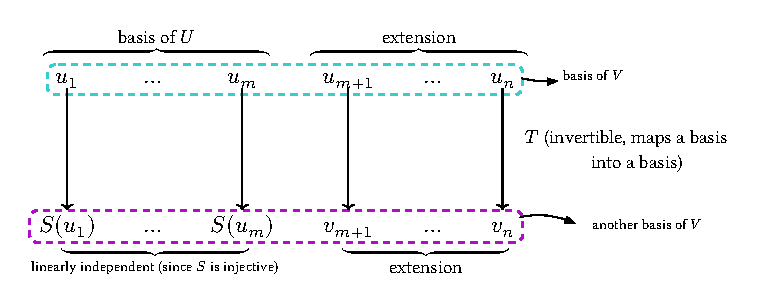
\includegraphics{plot_fletcher/plot_8_a.pdf}
   \end{figure}
   \newpage
   \begin{enumerate}[start=2]
      \item Suppose $V, W$ are finite-dimensional and $T_{1}, T_{2} \in \mathcal{L}(V, W)$. Prove that $\operatorname{null} T_{1} = \operatorname{null} T_{2}$ if and only if there exists an invertible operator $S \in \mathcal{L}(W)$ such that $T_{1}=S T_{2}$.
   \end{enumerate}
   Hint for (b): 
   \begin{figure}[htbp]
      \centering
      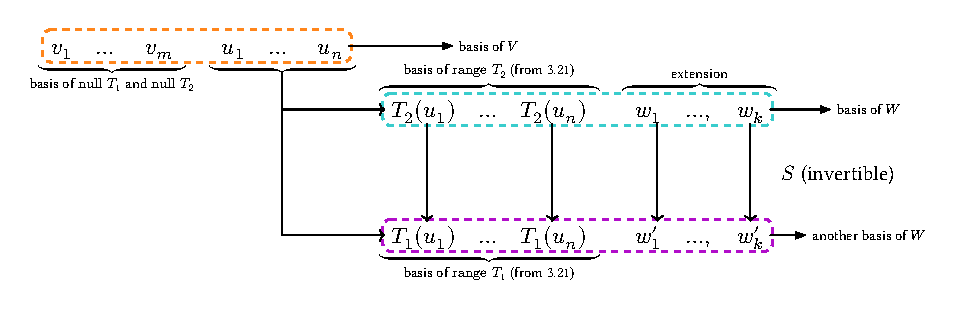
\includegraphics[scale=0.9]{plot_fletcher/plot_8_b.pdf}
   \end{figure}
   \newpage
  \item Suppose $V$ and $W$ are finite-dimensional and $T \in \mathcal{L}(V, W)$. Prove that $\operatorname{dim} \operatorname{range} T = 1$ if and only if there exist a basis of $V$ and a basis of $W$ such that with respect to these bases, all entries of the matrix representation $\mathcal{M}(T)$ equal $1$.
  \newpage
  \item Suppose that $V$ is a vector space. Show that $V$ and $\mathcal{L}(\mathbb{F}, V)$ are isomorphic vector spaces. ({\bf Note}: $V$ is not necessarily finite-dimensional, so you can't utilize the dimension test, and you should try to construct an isomorphic linear map.)
\end{enumerate}

\end{document}
